\chapter{Background}

\label{ch:background}
% \todo[inline, backgroundcolor=kth-lightblue]{Bakgrund}

% \todo[inline]{When you do your literature study, you should have a nearly complete Chapters 1 and 2.\\
% You may also find it convenient to introduce the future work section into your report early – so that you can put things that you think about but decide not to do now into this section.\\
% Note that later you can move things between this future work section and what you have done as you may change your mind about what to do now versus what to put off to future work.
% }
% \todo[inline]{What does a reader (another x student -- where x is your study line) need to know to understand your report?
% What have others already done? (This is the “related work”.) Explain what and
% how prior work / prior research will be applied on or used in the degree
% project /work (described in this thesis). Explain why and what is not used in
% the degree project and give valid reasons for rejecting the work/research.}

% This chapter provides basic background information about xxx. Additionally, this chapter describes xxx. The chapter also describes related work xxxx.



% \todo[inline, backgroundcolor=kth-lightblue]{Vilken viktig litteratur och
  % (forsknings-)artiklar har du studerat inom området (litteraturstudie)? }

This chapter presents concepts and information that is relevant for understanding, implementing, and evaluating FFS. We first present the idea of inode-based filesystems and how data is stored in a filesystem. Following is the introduction of Filesystem in Userspace (FUSE) which will be used to implement the filesystem. Later sections present background information about Twitter and the potential threat adversaries of the filesystem. 

\section{Filesystems}
Filesystems are used to store data on for instance a hard drive of a computer on in the cloud. Google Drive is a filesystem that enables user to save their data online up to 15 GB for free\cite{CloudStorageWork} using their clusters of distributed storage devices, meaning that the data is saved on theirs servers which can be located wherever\cite{DistributedStorageWhat}. Paying customers can achieve higher amount of storage using the service.

A deniable filesystem is a system that does not expose files stored on this system without credentials - neither how many files are stored, their sizes, their content or even if there exists any files on the filesystem\cite{petersDEFYDeniableFile2014}. This is useful if for example one is to be exposed to an audit of their data by a totalitarian regim where they don't even want to disclose that they have data.

A unix filesystem uses a data structure called an \textit{inode}. An inode keeps track of the metadata for the files in the filesystem, and a directory simply contains the file names, and each files/directory's inode id. Using a lookup, the system can then learn about the file - where it is located, for instance how big it is, as can be seen in Figure~\ref{fig:inode_diag} (\textbf{CITATION NEEDED}). Each inode entry can contain any number of metadata information which might be relevant for the system, such as creation time and last updated.

\begin{figure}[!ht]
	\begin{center}
	  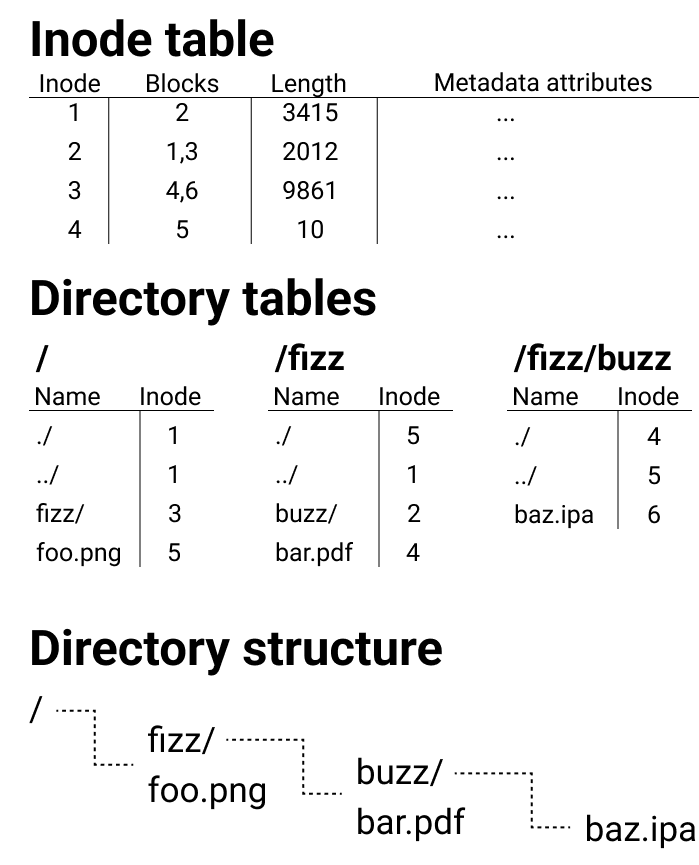
\includegraphics[width=0.8\textwidth]{figures/inode_diagram.png}
	\end{center}
	\caption{Basic structure of inode based filesystem}
	\label{fig:inode_diag}
\end{figure}

Looking at the 4 main file systems of windows, they all have many, sometimes different, functionalities such as links and named streams as well limitations such as a defined theoretical maximum file size\cite{mikbenFileSystemFunctionality}. This is set to 16 exbibytes for NTFS, exFAT and UDF, and for FAT32 it is set to 4 gigabytes. 

\section{FUSE}
\gls{FUSE} is a library that provides an interface to create filesystems in userspace rather than in kernel space which is otherwise often considered the standard when writing commercial filesystems\,\cite{Libfuse2021}. The reason to implement a filesystem in kernel space is that it leads to faster system calls than when writing a filesystem in userspace. However, while filesystems written with \gls{FUSE} are generally slower than \mbox{kernel-based} filesystems, using \gls{FUSE} simplifies the process of creating filesystems. macFUSE is a port of \gls{FUSE} that operates on Apple's macOS operating system and it extends the \gls{FUSE} \gls{API}\,\cite{HomeMacFUSE}. macFUSE provides an \gls{API} for C and Objective C.
% TODO: MAYBE add about this "If you use these extensions, then how is it portable to \mbox{non-MAC} systems?". Cannot find anything online though

Figure~\ref{fig:fuse_desc} presents an overview how \gls{FUSE} works. \gls{FUSE} consists of a kernel space part and a userspace part that perform different tasks\,\cite{vangoorFUSENotFUSE2017}. The kernel part of \gls{FUSE} operates with the \gls{VFS} which is a layer in both the Linux kernel and the macOS kernel that exposes a filesystem interface for userspace applications\,\cite{goochOverviewLinuxVirtual, singhMacOSInternals2006}. The \gls{VFS} interface is independent of the underlying filesystem and is an abstraction of the underlying filesystem operations which can be used on any filesystem the \gls{VFS} supports. The userspace part of \gls{FUSE} communicates with the kernel space part through a block device. Operations on a mounted \gls{FUSE} filesystem are sent to the \gls{VFS} from the user application, which is then sent to the kernel part of \gls{FUSE}. If needed, the operations are transmitted to the userspace part of \gls{FUSE} where the operation is handled and a response is sent back to the \gls{VFS} and the user application through the \gls{FUSE} kernel module. However, some actions can be handled by the \gls{FUSE} kernel module directly, such as if the file is cached in the kernel part of \gls{FUSE}\,\cite{vangoorFUSENotFUSE2017}. The response is then sent back to the user application from the kernel module through the \gls{VFS}.

\begin{figure}[!ht]
	\begin{center}
	  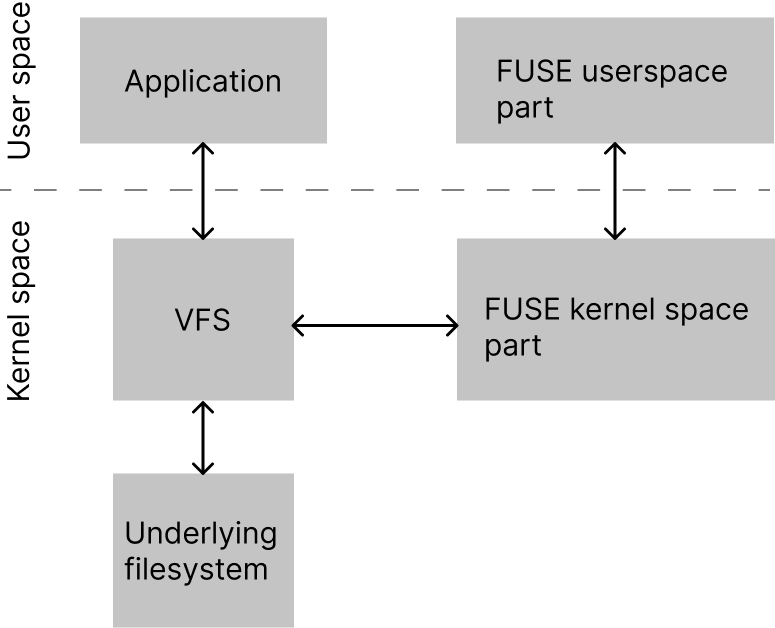
\includegraphics[width=0.5\textwidth]{figures/fuse_description.png}
	\end{center}
	\caption{Simple visualization of how \gls{FUSE} operations are executed}
	\label{fig:fuse_desc}
\end{figure}

\section{Online web services}
\label{sec:ows}
This section presents two online web services (OWSs), Twitter and Flickr, where one can create free-tier accounts. On both of these OWSs, free-tier accounts can make numerous of posts for free. The OWSs provide free-to-use Application Programming Interfaces (APIs) for non-commercial development. 

\subsection{Twitter}
\label{subsec:ows_twitter}
Twitter is a micro-blog online where users can sign up for a free account and create public posts (tweets) using text, images, and videos. Each post has an unique id associated with it\,\cite{twitterTwitterIDs}. Text posts are limited to $280$ characters while images can be up to \SI{5}{\mega\byte} and videos up to \SI{512}{\mega\byte}\,\cite{MediaBestPractices}. An post with images can contain up to 4 images in one post. There is also a possibility to send private messages to other accounts, where each message can contain up to $10\,000$ characters and the same limitations on files. However, direct messages older than $30$ days are not possible to retrieve through Twitter's API\,\cite{RetrievingOlder302018}. It is possible to create threads of Twitter posts where multiple tweets can be associated in chronological order.

Twitter's API defines technical limits of how many times certain actions can be executed by an user\,\cite{UnderstandingTwitterLimits}. A maximum of $2\,400$ tweets can be sent per day, and the limit is further broken down into smaller limits at semi-hourly intervals. Hitting a limit means that the user account no longer can perform the actions that the limit represents until the time period has elapsed.

\subsection{Flickr}
\label{subsec:ows_flickr}
Flickr is a public image and video hosting service, used to store and share photos and videos. Unlike Twitter, a post on Flickr is based on the image or video. The post can, optionally, have a title, a description, or both. However, the post must have exactly one photo or video. Flickr supports multiple image and video formats, including PNG and MP4\,\cite{FlickrUploadRequirements2022}. Restrictions are set for each post, depending on the media type. Images uploaded to Flickr can be a maximum of \SI{200}{\mega\byte} and a video can be maximum of \SI{1}{\giga\byte}. Further, free-tier accounts can only have total of 1\,000 photos or videos on their account. A Flickr Pro account has unlimited storage on Flickr, but is still subject to the per-item limit of \SI{200}{\mega\byte} and \SI{1}{\giga\byte} for images and videos, respectively\,\cite{flickrinc.UpgradeEverythingYou}. Flickr Pro costs between 7.49€ to 5.49€ per month, depending on the subscription time the user signs up for. The description of a post has a limit of 65535 characters according to Shhexy Corin\,\cite{FlickrHelpForum2009}. This has been verified through testing. The title of a post has also been discovered to have a limit of 255 characters through testing.

The images and videos uploaded to Flickr is stored in its original form \textbf{without any compression}, and can be downloaded by the user as the same file as was uploaded\cite{flickrinc.DownloadPermissions}. Flickr also stores other formats of the file, such as thumbnails. User accounts can restrict who, other than themselves, can download the original image. The original video can only be downloaded by the user\,\cite{flickrinc.DownloadPermissions}. Flickr do not state if it will always be possible to download the original versions of the file. Further, Flickr states that it retains the right to remove user content from the service at any time\,\cite{flickrinc.FlickrTermsConditions2020}.

The Flickr API defines a query limit of 3\,600 requests per hour, per application, across all API calls\,\cite{flickrinc.FlickrFlickrDeveloper}. However, according to Sam Judson in 2013, this is not a hard limit\,\cite{WhatAreAPI2013}. There is no official information from Flickr of what happens if you break the hourly request limit. The Flickr API states that the API is monitored on other factors as well\,\cite{flickrinc.FlickrFlickrDeveloper}. If abuse is detected, Flickr reserves the right to revoke API keys.

\section{Cryptography}
\label{sec:back_crypto}
The Advanced Encryption Standard (AES) is a encryption standard established by the U.S. National Institute of Standards and Technology (NIST), more specificity specifying the Rijndael block cipher\,\cite{kumarvermaPerformanceAnalysisRC62012}. AES is a symmetrical cipher, meaning that the same key is used for encryption and decryption. AES is used to make the data confidential, so that no one except the person with the key can access the unencrypted data. AES produces 128-bit encrypted cipher blocks, and supports key sizes of 128 bits, 192 bits, or 256 bits. The security of AES has been heavily researched since its introduction in the early 2000s, and literature has found it is well resistant to quantum attacks as well\,\cite{bonnetainQuantumSecurityAnalysis2019}.

While AES is a good standard for the confidentiality of the data, confidentiality is often not enough to secure the data\,\cite{rosswallrabensteinWhenItComes2021}. Importance of ensuring the authenticity of the data is also high. This means that we want to know that the data has not been modified since it was encrypted. This problem can be solved by using authenticated encryption\,\cite{khovratovichAnswerWhyShould2013}. The Galois/counter mode of operation (GCM) is a block cipher mode of operation which provides authenticated encryption\,\cite{mcgrewGaloisCounterMode2004}. GCM can be used with AES to provide secure, authenticated encryption of data. To encrypt using GCM, the encryption function requires a key, a randomized Initialization Vector (IV) and the data to encrypt. The output is the encrypted cipher text and an authentication tag. The decryption function of GCM requires the same key and IV as was used as input in the encryption function, as well as the authentication tag and the cipher text received as output by the encrypting function. Further, both the encryption function and the decryption support Additional authentication data (ADD) to be provided. ADD is data that should be authenticated, but not encrypted. If ADD is provided to the encryption function, it must also be provided to the decryption function.

The key used when encrypting using AES is often derived from a password that the user provides. Password-Based Key Derivation Functions (PBKDFs) are functions that can be used to derive a key used for, for instance, AES. The input to a PBKDF is a secret, such as a password\,\cite{kodwaniSecurityKeyDerivation2021}. An example of a PBKDF schema is the hashed message authentication code (HMAC) based key derivation functions (HKDF) presented by \citeauthor{krawczykCryptographicExtractionKey2010}\,\cite{krawczykCryptographicExtractionKey2010}\cite{krawczykHMACbasedExtractandExpandKey2010} which utilizes a hashing algorithm that provide a pseudo-random key. HKDF supports multiple hashing algorithms. The security of HKDF is partially dependent on the security of the hashing algorithm used. A well-defined suit of hashing algorithms is the Secure Hash Algorithms (SHA), which covers, among other hash functions, SHA-256 \cite{hansenUSSecureHash2011}. SHA-256 is a cryptographic hash function which outputs a 256-bit pseudo-random cipher from its input, which can, for instance, be a password. Further, HKDF uses a salt to improve the security of the provided secret. The salt is random data used to further diffuse the produced key, making two keys with the same secret but different salts, different\,\cite{ariasAddingSaltHashing2021}. The salt does not have to be secret, and is sometimes stored with the produced cipher so that the decryption function easily can re-use the salt when deriving the decryption key. If the key used for encryption and the key used for decryption are derived using different salts, the keys will differ and the cipher cannot be decrypted.


\section{Threats}
To consider a filesystem secure it is important to imagine different potential adversaries who might attack the system. Considering that FFS has no real control of the data stored on the different services, all the data must be considered to be stored in an insecure system. Even if we could hide the posts made on for instance Twitter by making the profile private, we must still consider that Twitter themselves could be an adversary or that they could potentially give out information, such as tweets or direct messages, to entities such as the police. In fact, Twitter's privacy policy mentions that they may share, disclose, and preserve personal information and content posted on the service, even after account deletion for up to $18$ months\,\cite{TwitterPrivacyPolicy}. Therefore, to achieve security the data stored must always be encrypted. We assume that an adversary has access to all knowledge about FFS, including how the data is converted, encrypted, and posted. We also assume they know which websites and accounts that could post data from the filesystem - but we assume they do \textbf{not} have the decryption key. There are multiple secure ways of encrypting data, including AES which is one of the faster and more secure encryption algorithms\,\cite{mahajanStudyEncryptionAlgorithms2013}. However, even though the data is encrypted, other properties such as your IP address can be compromised which can expose the user's identity. The problem of these other sources of information external to FFS is not addressed in FFS but remains for future work.

Other than adversaries for FFS, we might also imagine that the underlying services might face attacks that can potentially harm the security of the system or even cause the service to go offline, potentially indefinitely. One solution is to use redundancy - by duplicating the data over multiple services, we can more confidently believe that our data will be accessible as the probability of all services going offline at the same time is lower.

The deniability of FFS is an important aspect of the filesystem. Potential threat adversaries are agents that the user is trying to hide the data from, such as governing states. For the system to be deniable, an adversary should not be able to gain any information about anything about the potential data in the system, this includes even the existence of data. When the filesystem is unmounted there should be no trace of the filesystem ever being present in the device. We will assume that an adversary is competent and can analyze the software and hardware completely.